\documentclass{beamer}

\mode<presentation>

\usetheme{Pittsburgh}


\usepackage[utf8]{inputenc}
\usepackage{ beamerthemesplit}
\usepackage{caption}
\usepackage{adjustbox}
\newtheorem*{teor}{Teorema}
\newtheorem*{teort}{Teorema de Tibor Radó}
\newtheorem*{lema}{Lema}
\newtheorem*{ejem}{Ejemplos}
\newtheorem*{prop}{Proposición}
\newtheorem*{defi}{Definición}

%\mode<handout>
{
\beamertemplatesolidbackgroundcolor{black!5}
}
\usepackage{amssymb,amsmath,amsfonts,graphicx,float,epsfig,enumerate}
\usepackage{amsopn}
\usepackage{fancyhdr}
\renewcommand{\figurename}{}

\renewcommand{\baselinestretch}{1}

% \newenvironment{flushenum}{
% \begin{enumerate}
%   \setlength{\leftmargin}{0pt}
% }{\end{enumerate}}

\sloppy

\parindent 0pt

%\usepackage[dark,tab]{beamerthemesidebar}

%\logo{\includegraphics[width=1cm,height=1cm]{logo.pdf}}

\title[Teorema de clasificación de superficies]{Teorema de clasificación de superficies topológicas}
\author[Rodrigo De Pool]{}
%\institute[UAM]{}
\date[]{Junio 2020}
\subject{}

%\AtBeginSubsection[]
%{
% \begin{frame}<beamer>
%    \frametitle{Plan of the talk}
%    \tableofcontents[currentsection,currentsubsection]
%  \end{frame}
% }

\newcommand{\oo}{$^{\mbox{\underline{\tiny o}}}$\hspace{2 mm}}

\definecolor{dark}{gray}{.5}
\definecolor{rosa_claro}{rgb}{1,0.9,0.9}
%\definecolor{azul_intenso}{rgb}{0,0.6,0.9}
\definecolor{azullito}{rgb}{0.4,0.5,0.9}
%\definecolor{amarillo_claro}{rgb}{1,1,0.7}
%\definecolor{gris_claro}{gray}{0.9}
\definecolor{uofsgreen}{rgb}{.125,.5,.25}

\usecolortheme[named=azullito]{structure} % Para cambiar el fondo de los frametitles

\begin{document}
%%%%%%%%%%%%%%%%%%%%%%%%%%%%%%%%%%%%%%%%%%%%%%%%%%%%%%%%%%%%%%%%%%%%%%%%%%%%%
%%%%% TITULO %%%%%%%%%
\frame{\titlepage}
 
%%%%%% DIAPOSITIVA 1 %%%%%%
\begin{frame}
\frametitle{Superficies topológicas}

\begin{block}{Superficie topológica}
\begin{itemize}
    \item Localmente homeomorfo a una bola en $\mathbb{R}^2$.
    \item Hausdorff, segundo numerable y conexo (*orientable).
\end{itemize}
\end{block}

Algunos ejemplos
\begin{figure}[htb]
\begin{center}
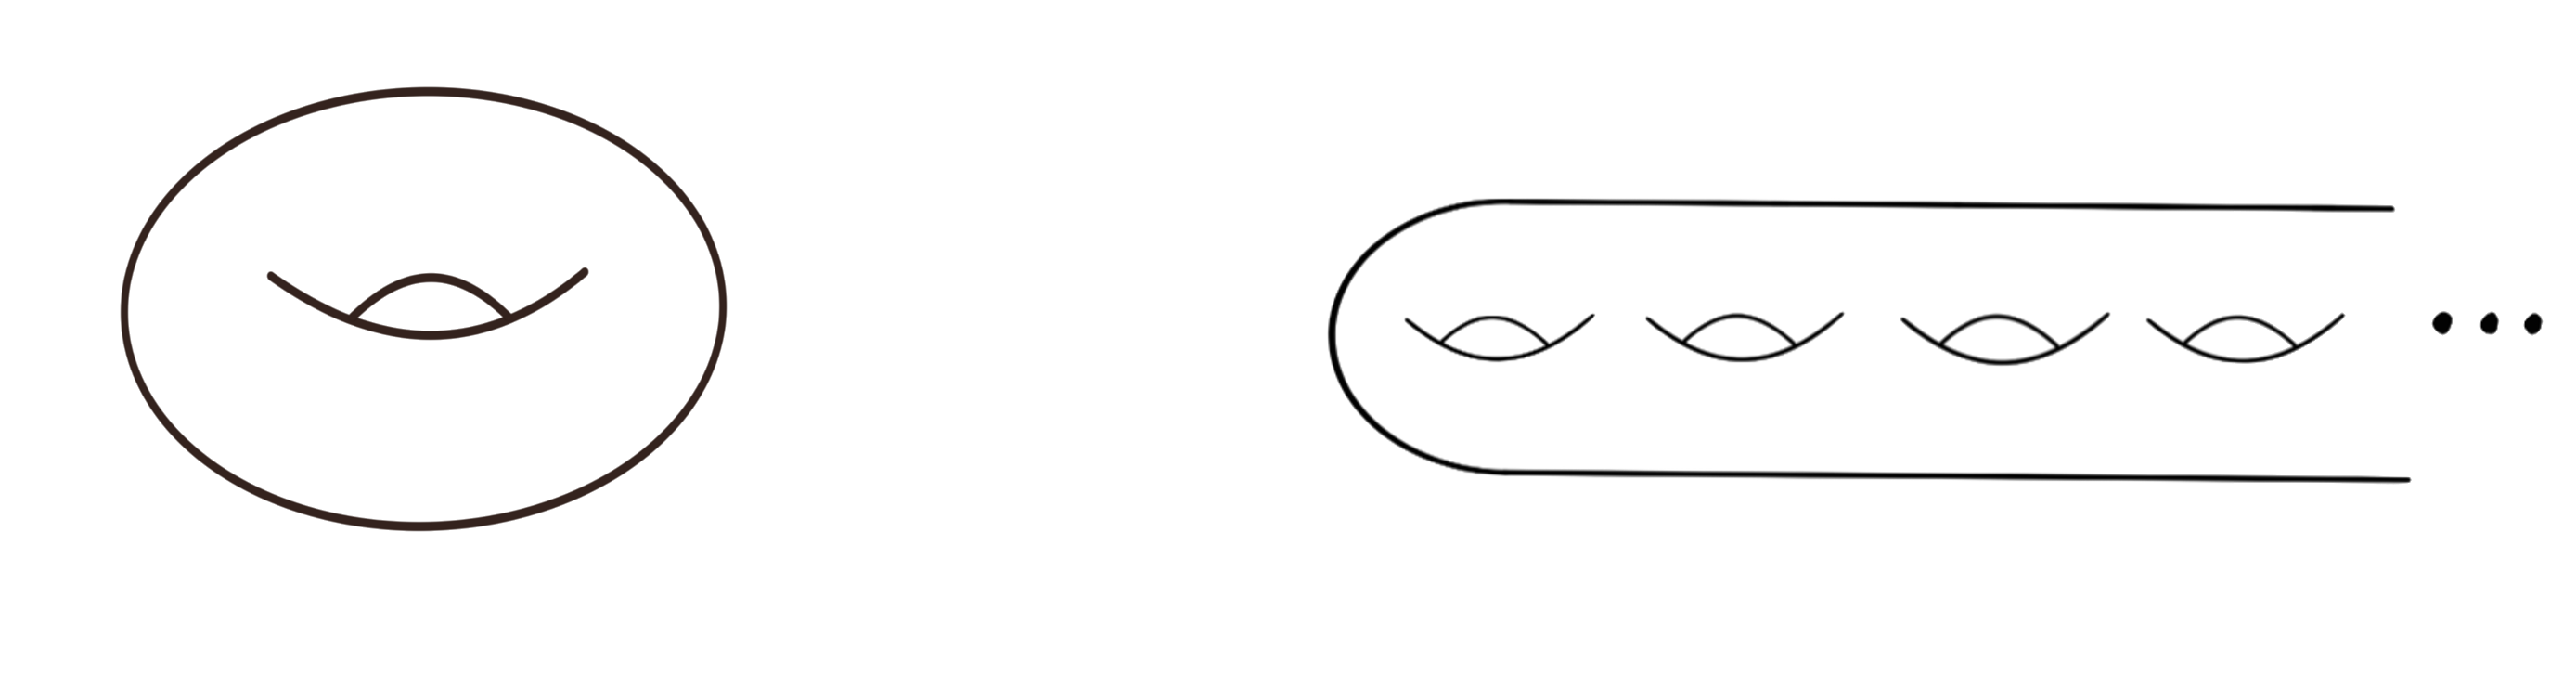
\includegraphics[width=3in,height=1in]{imagenes/diapo1.png} 
\end{center}
\end{figure}

\end{frame}

% DIAPO 2
\begin{frame}
\frametitle{Suma conexa}
\begin{block}{Suma conexa}
Operador entre superficies

\end{block}
\begin{figure}[htb]
\begin{center}
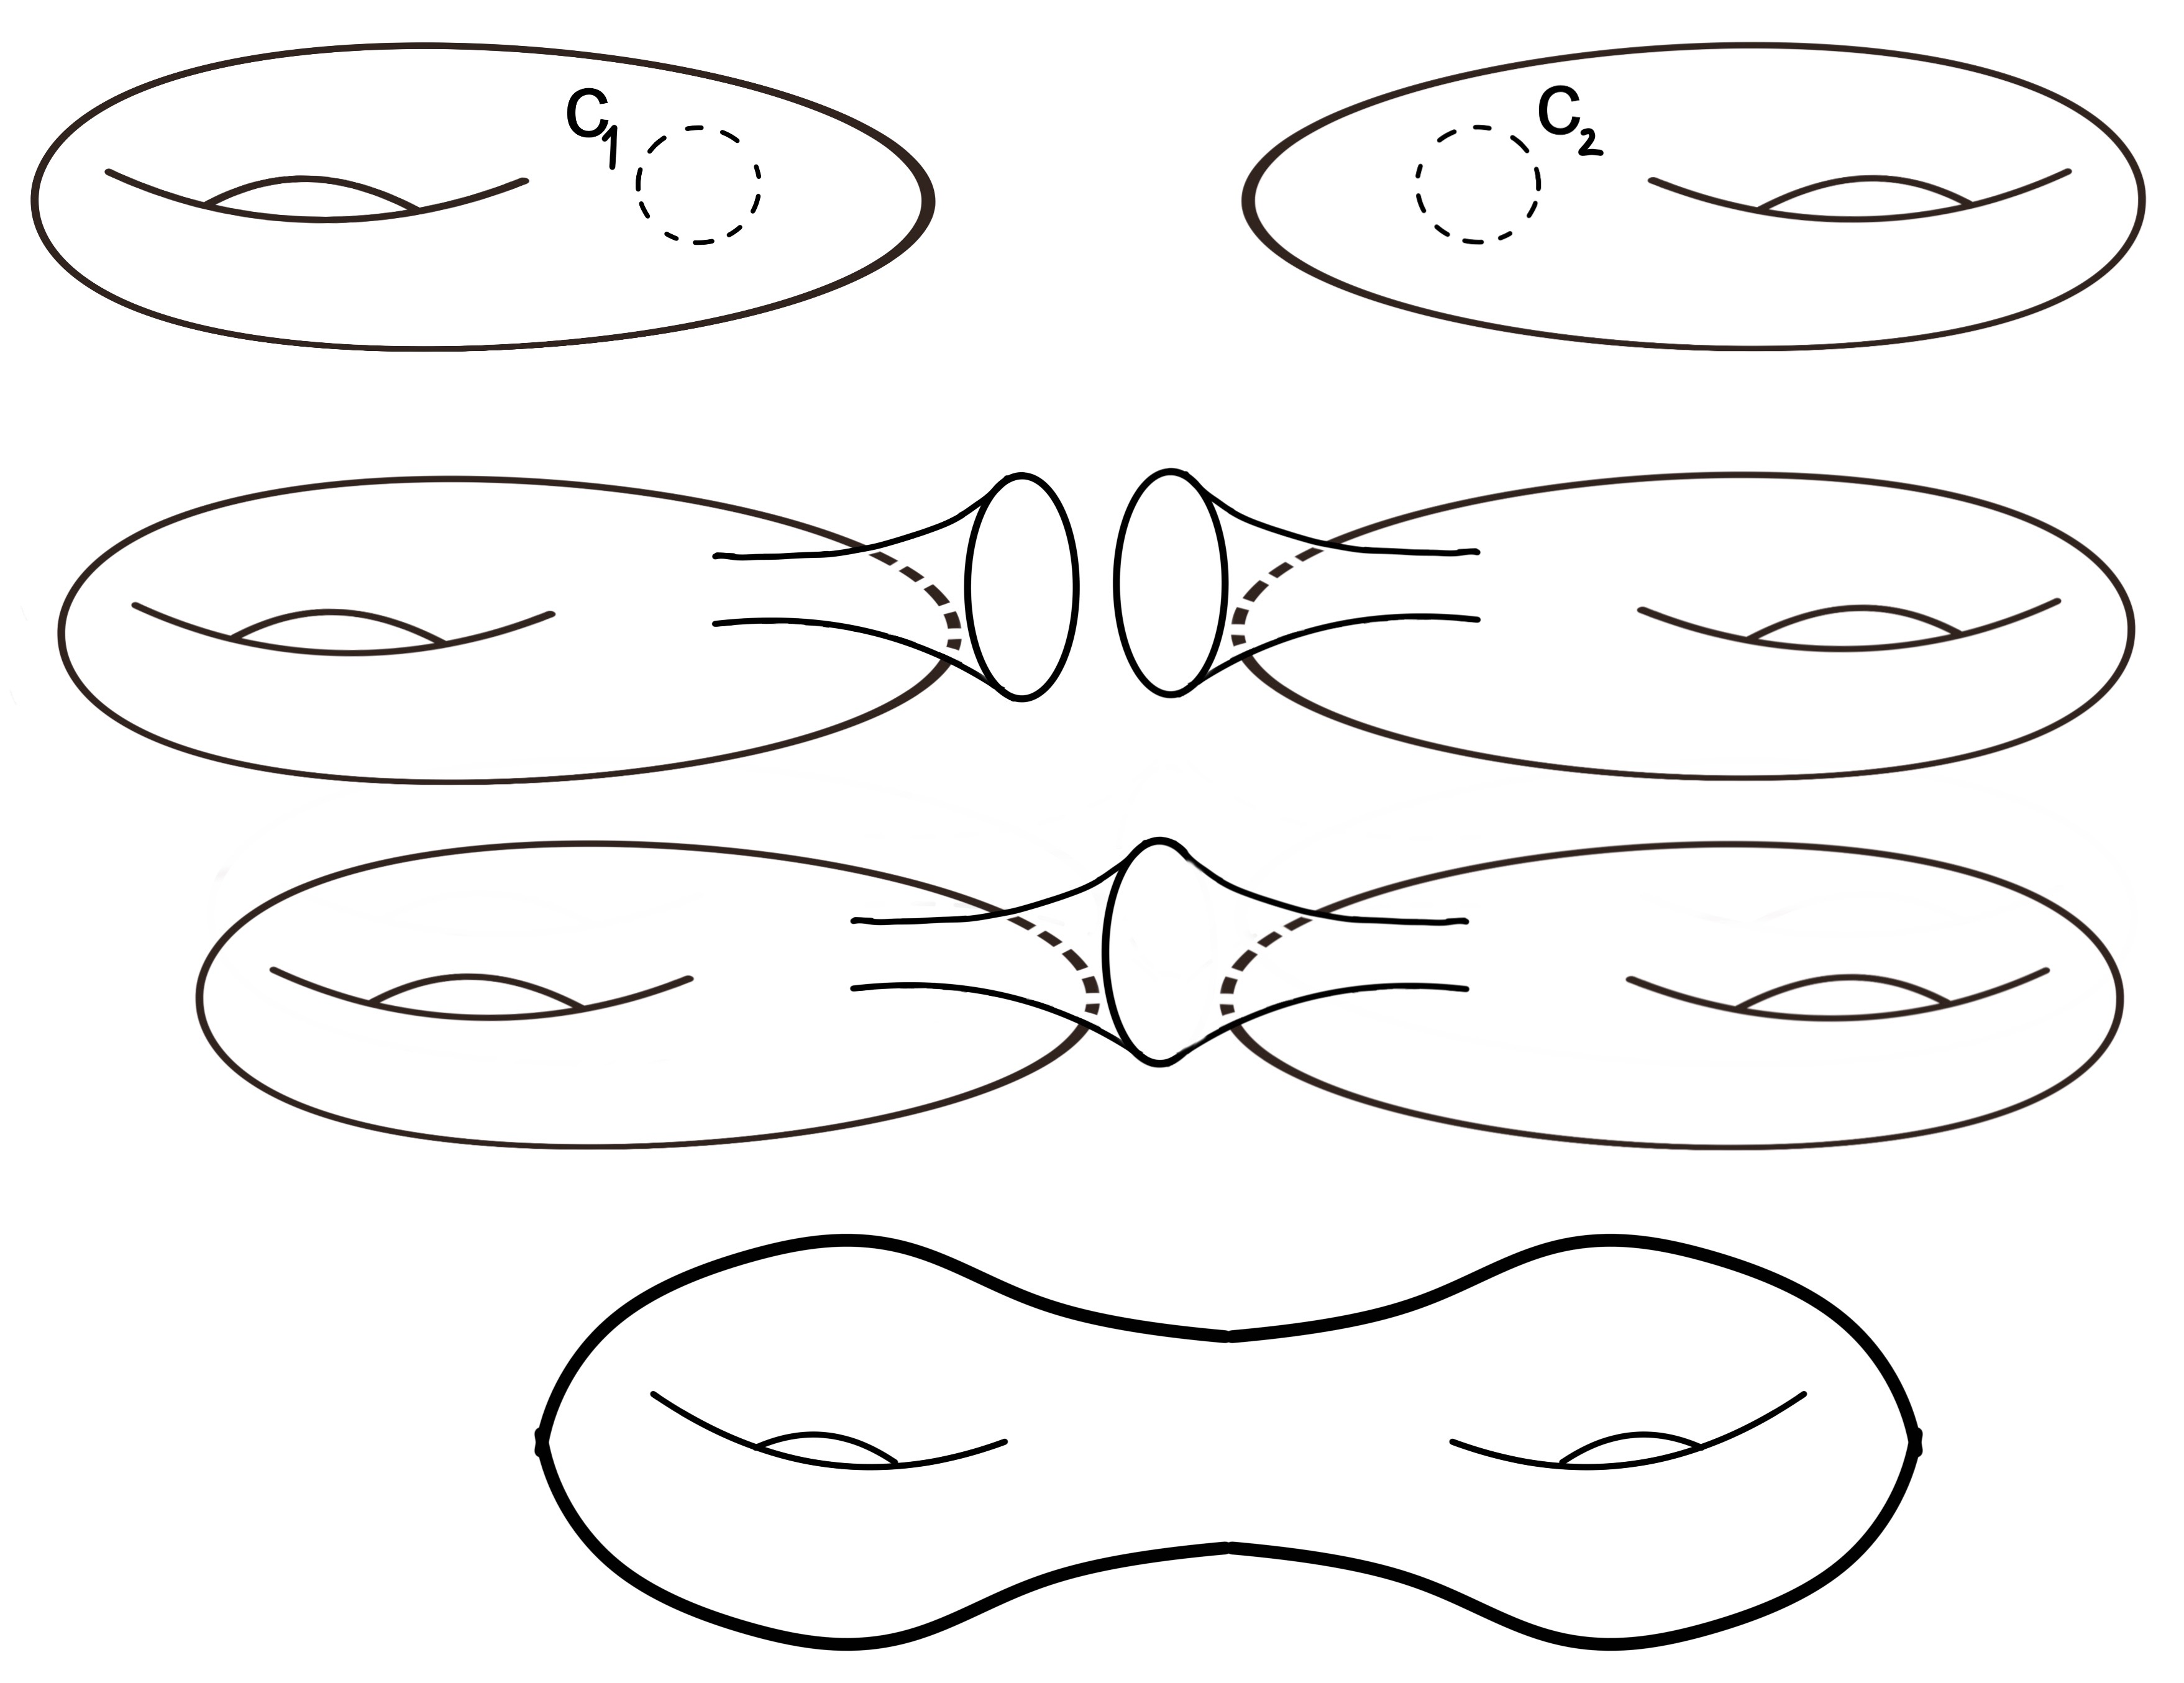
\includegraphics[width=2in,height=1.5in]{imagenes/sumaconexa_toros_R3.png} 
\end{center}
\end{figure}

\end{frame}

% Diapo 3
\begin{frame}
\frametitle{Ejemplos de suma conexa}
Toro y suma conexa de dos toros:
\begin{figure}[htb]
\begin{center}
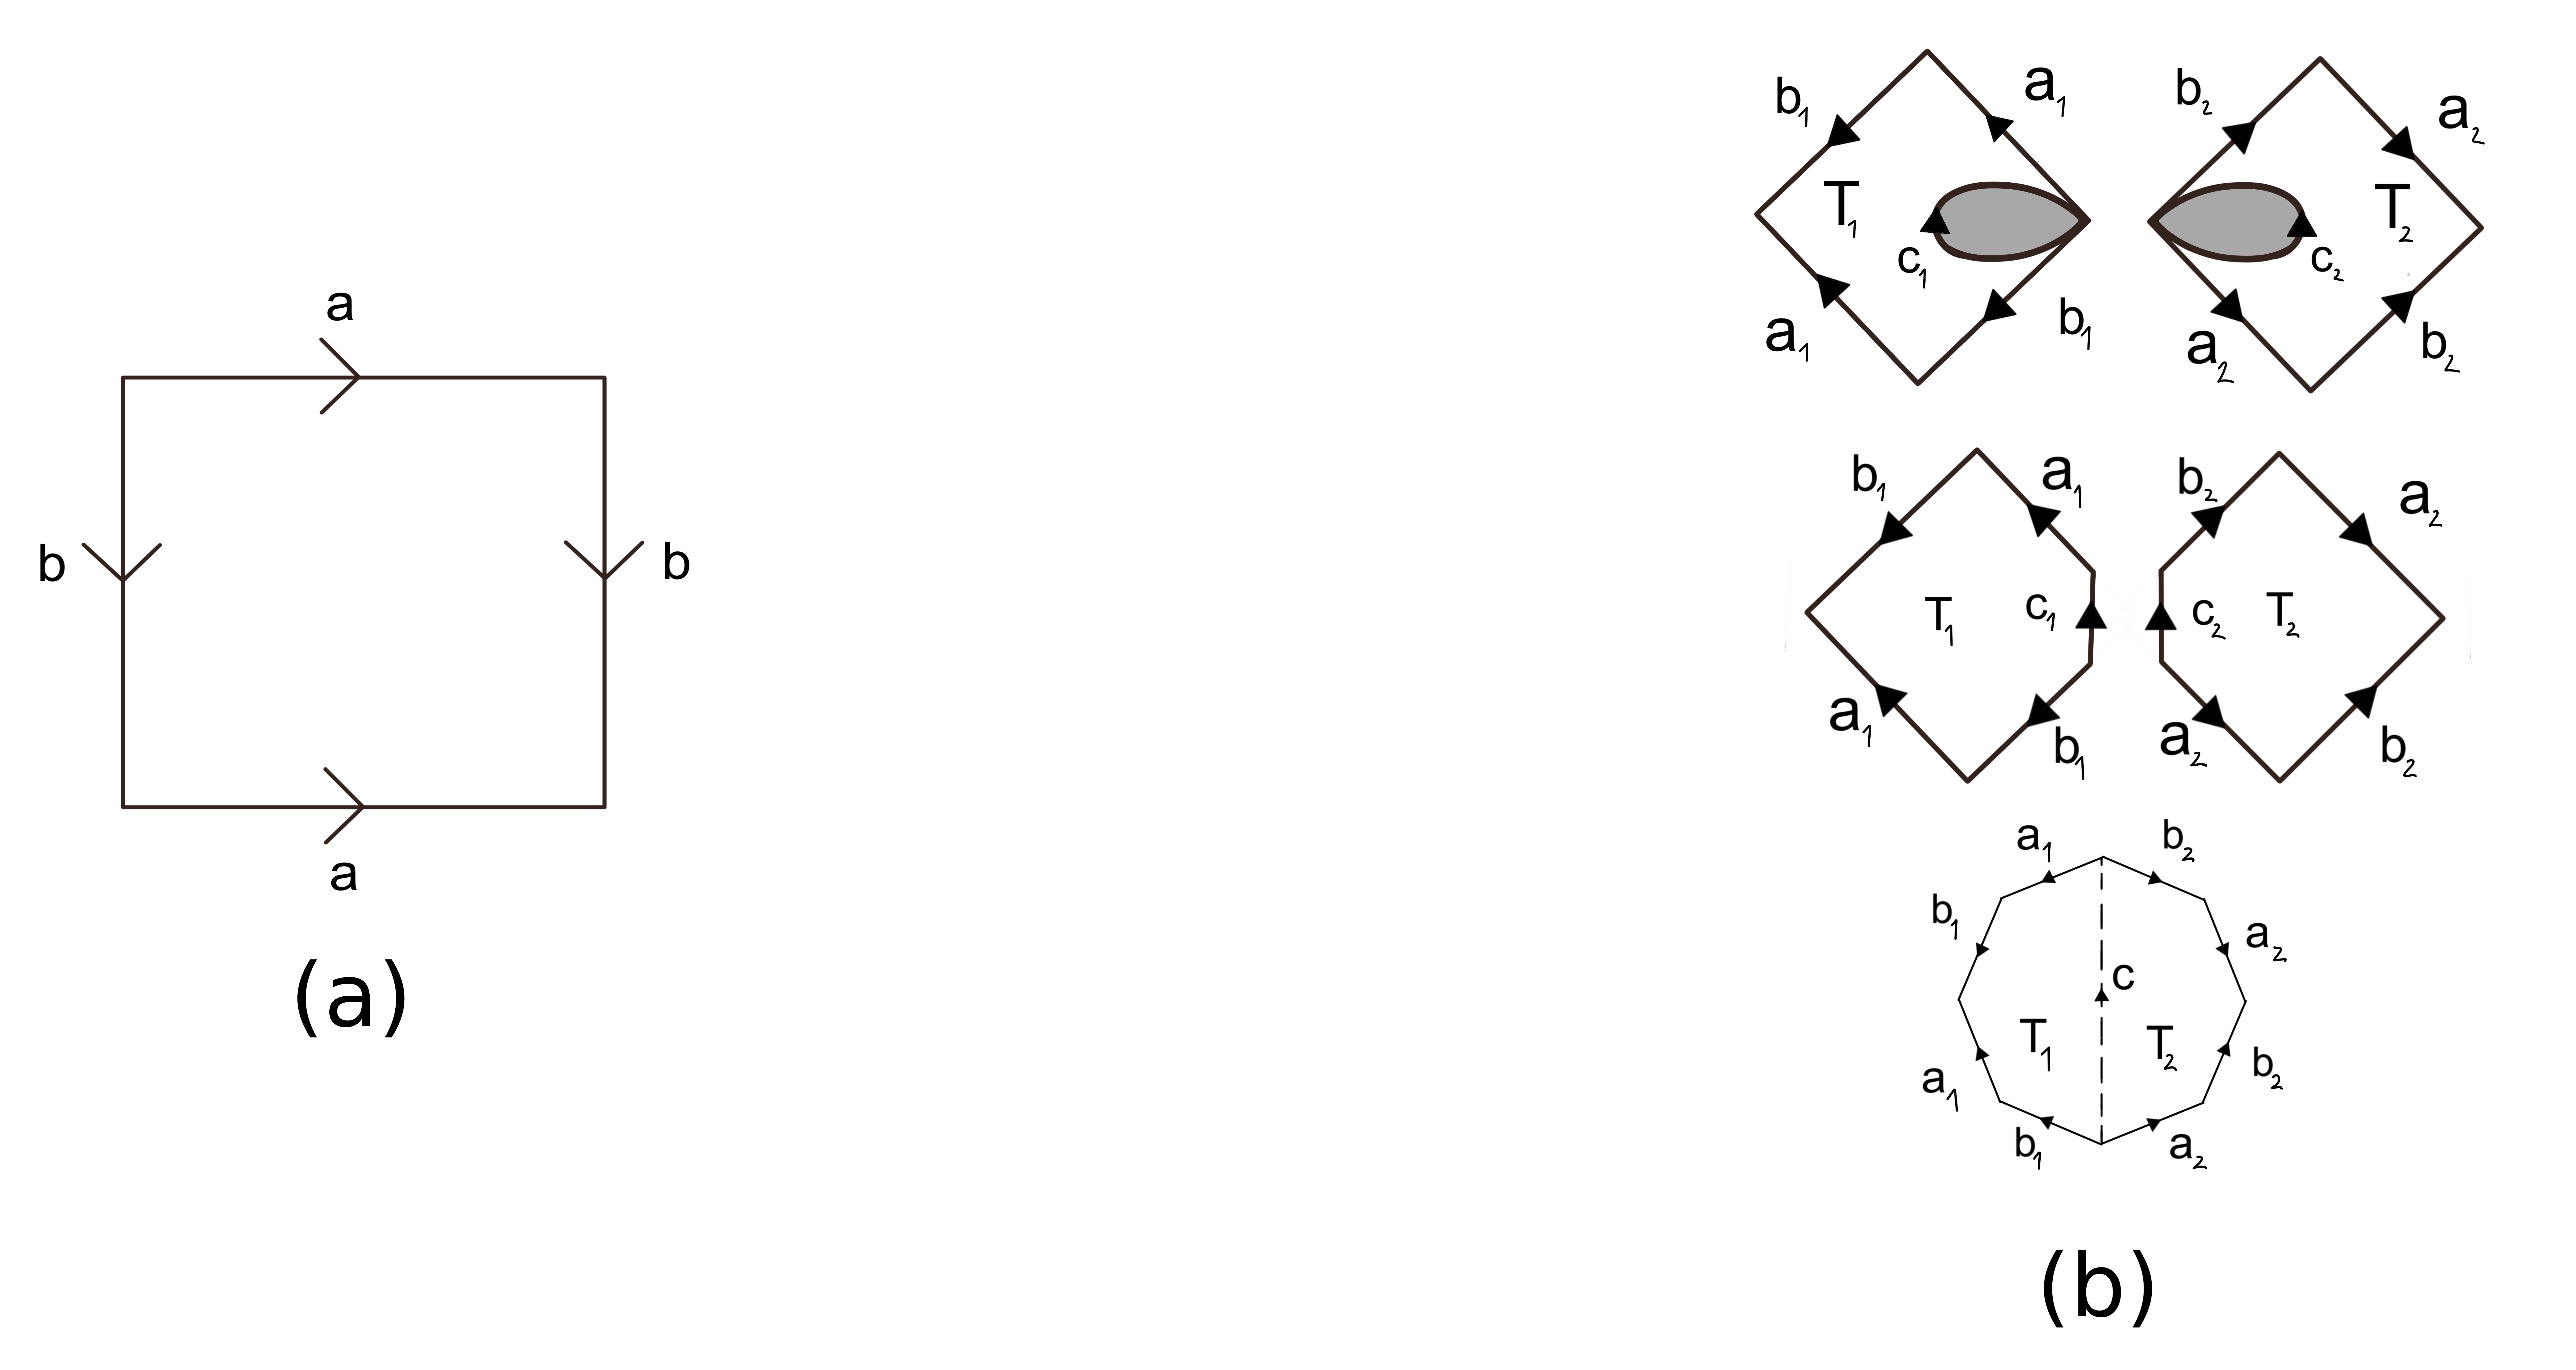
\includegraphics[width=3in,height=2in]{imagenes/sumaconexa1.png}
\end{center}
\end{figure}
\end{frame}


% Diapo 4
\begin{frame}
\frametitle{Clasificación de superficies compactas}
\begin{block}{Teorema de clasificación de superficies compactas}
Toda superficie compacta orientable es homeomorfa a una esfera o a una suma conexa de $n$ toros.
\end{block}

\begin{figure}[htb]
\begin{center}
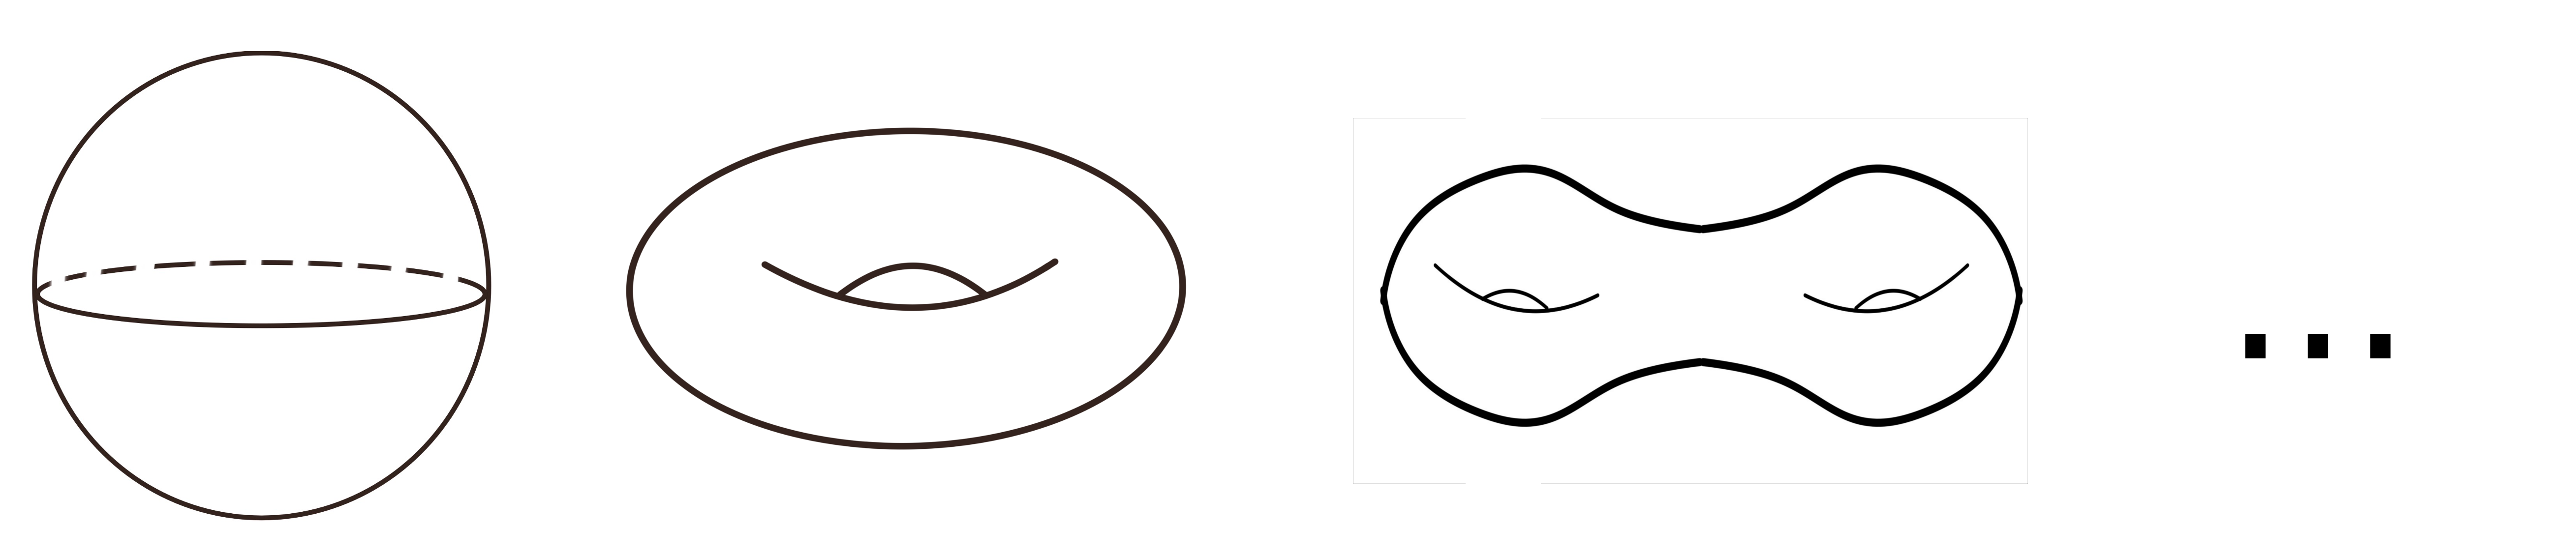
\includegraphics[width=4in,height=0.75in]{imagenes/diapo4.png} 
\end{center}
\end{figure}
\end{frame}

% Diapo 5
\begin{frame}
\frametitle{Triangulación}
\begin{block}{Teorema (Radó 1925)}
Toda superficie separable es triangulable.
\end{block}


\begin{figure}[htb]
\begin{center}
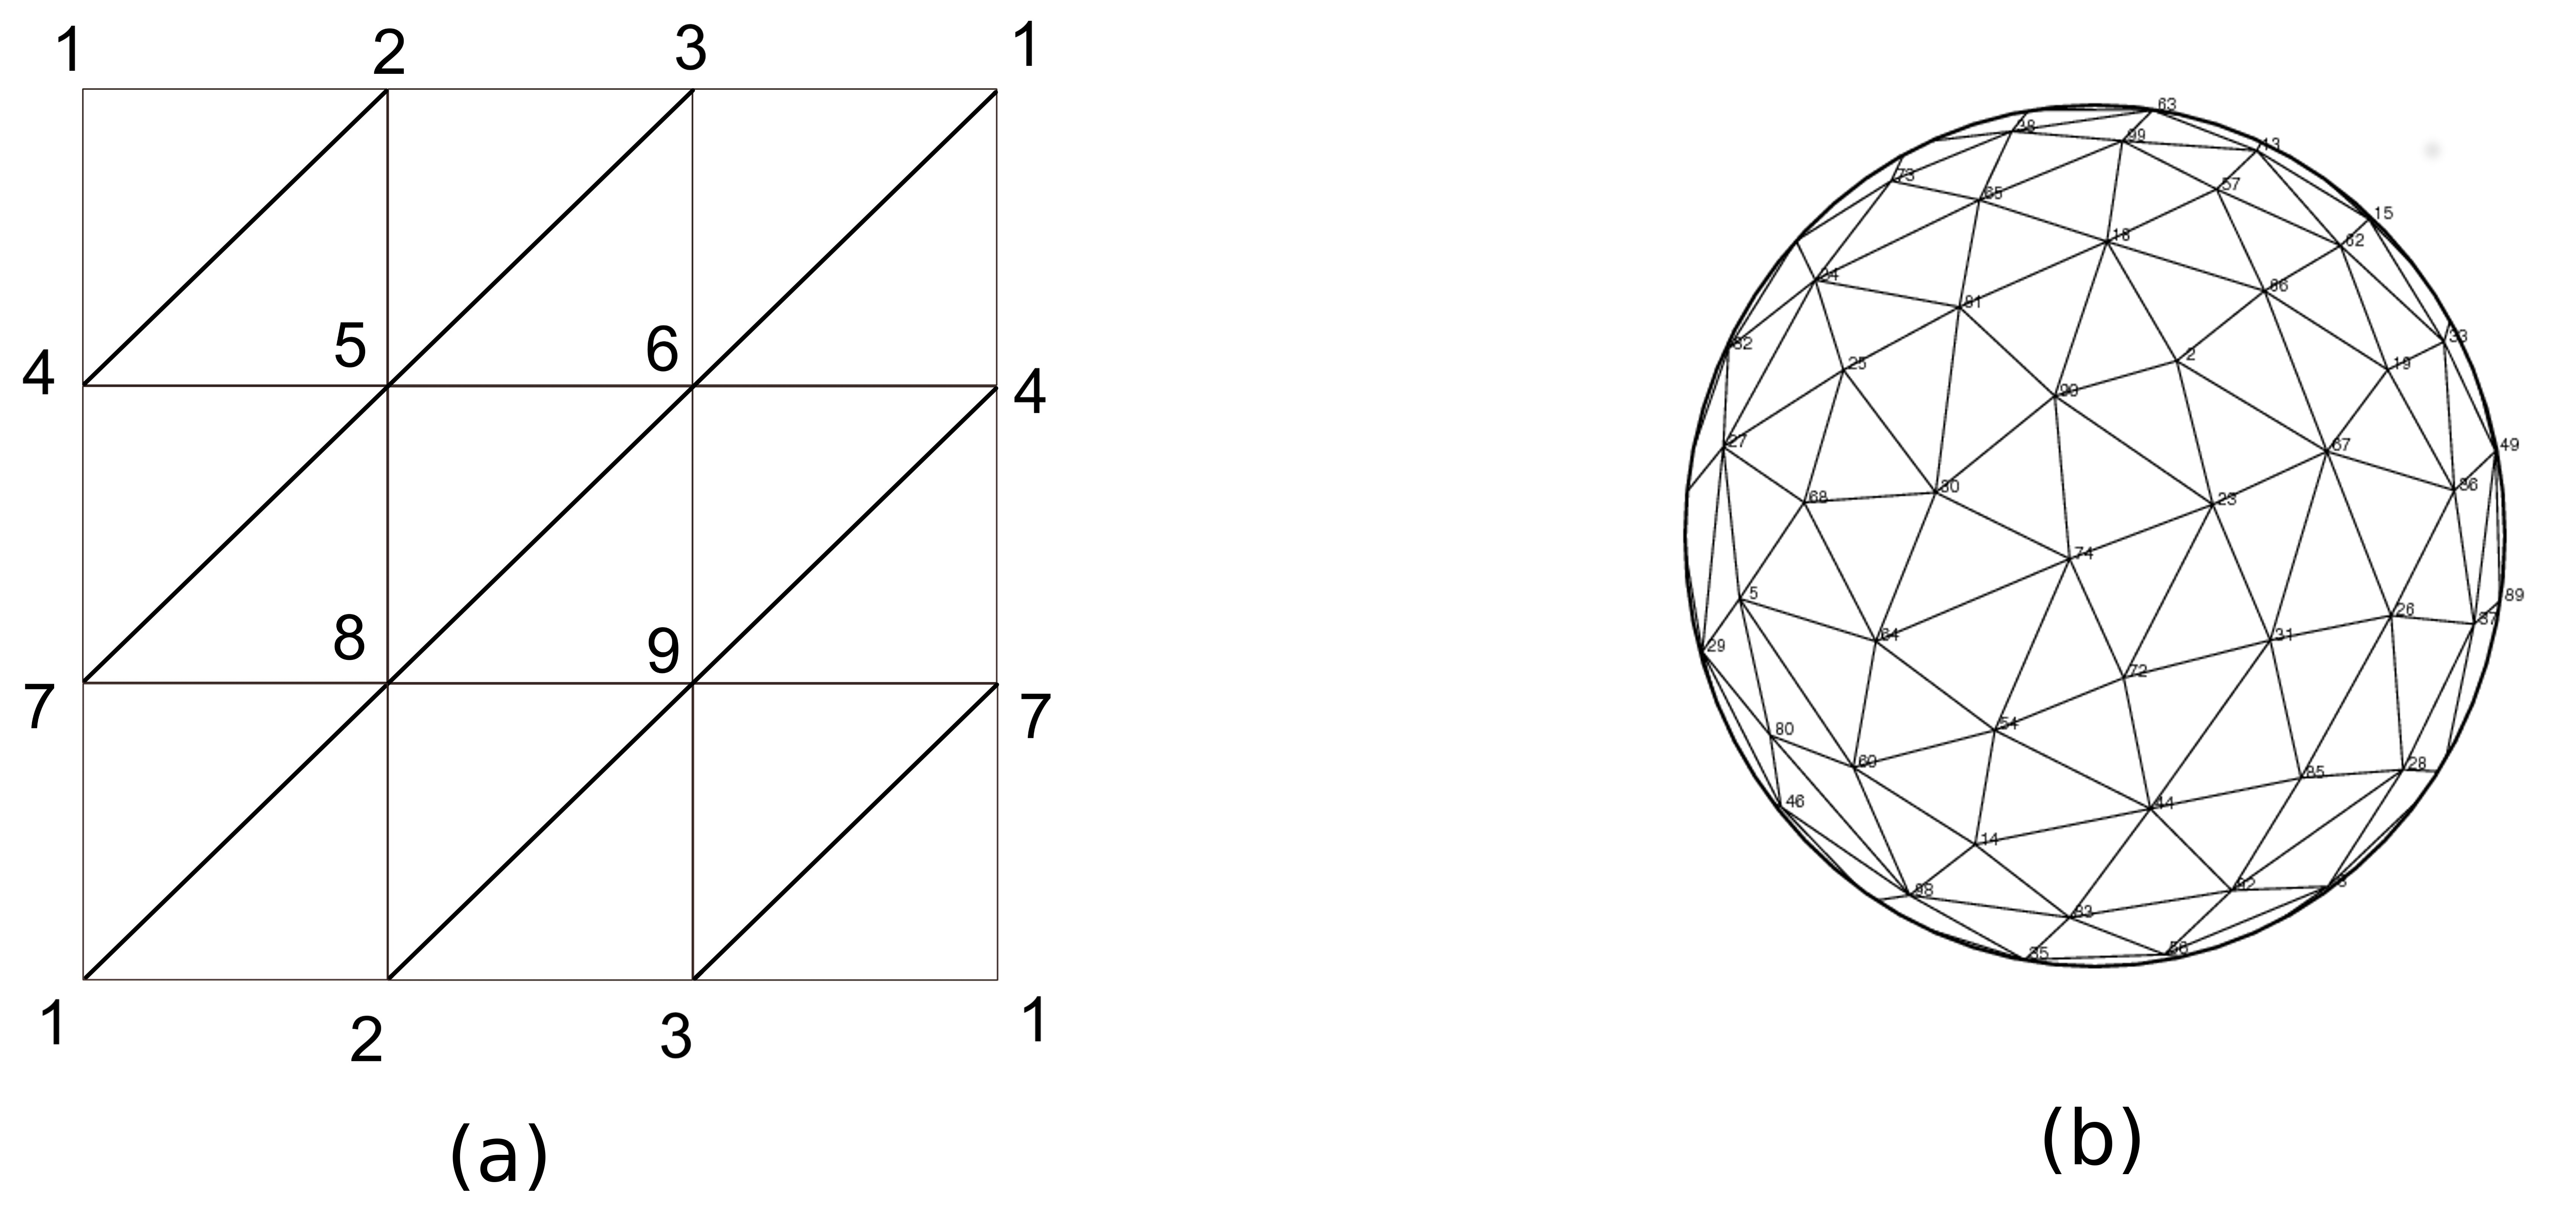
\includegraphics[width=2in,height=0.75in]{imagenes/diapo3.png} 
\caption{Toro y esfera triangulados.}
\end{center}
\end{figure}

\end{frame}


% Diapo 7

\begin{frame}
\frametitle{Idea de la demostración}

\begin{block}{Paso 1}
Se usa el resultado de Radó para expresar una superficie como un polígono con las aristas identificadas a pares.
\begin{figure}[htb]
\begin{center}
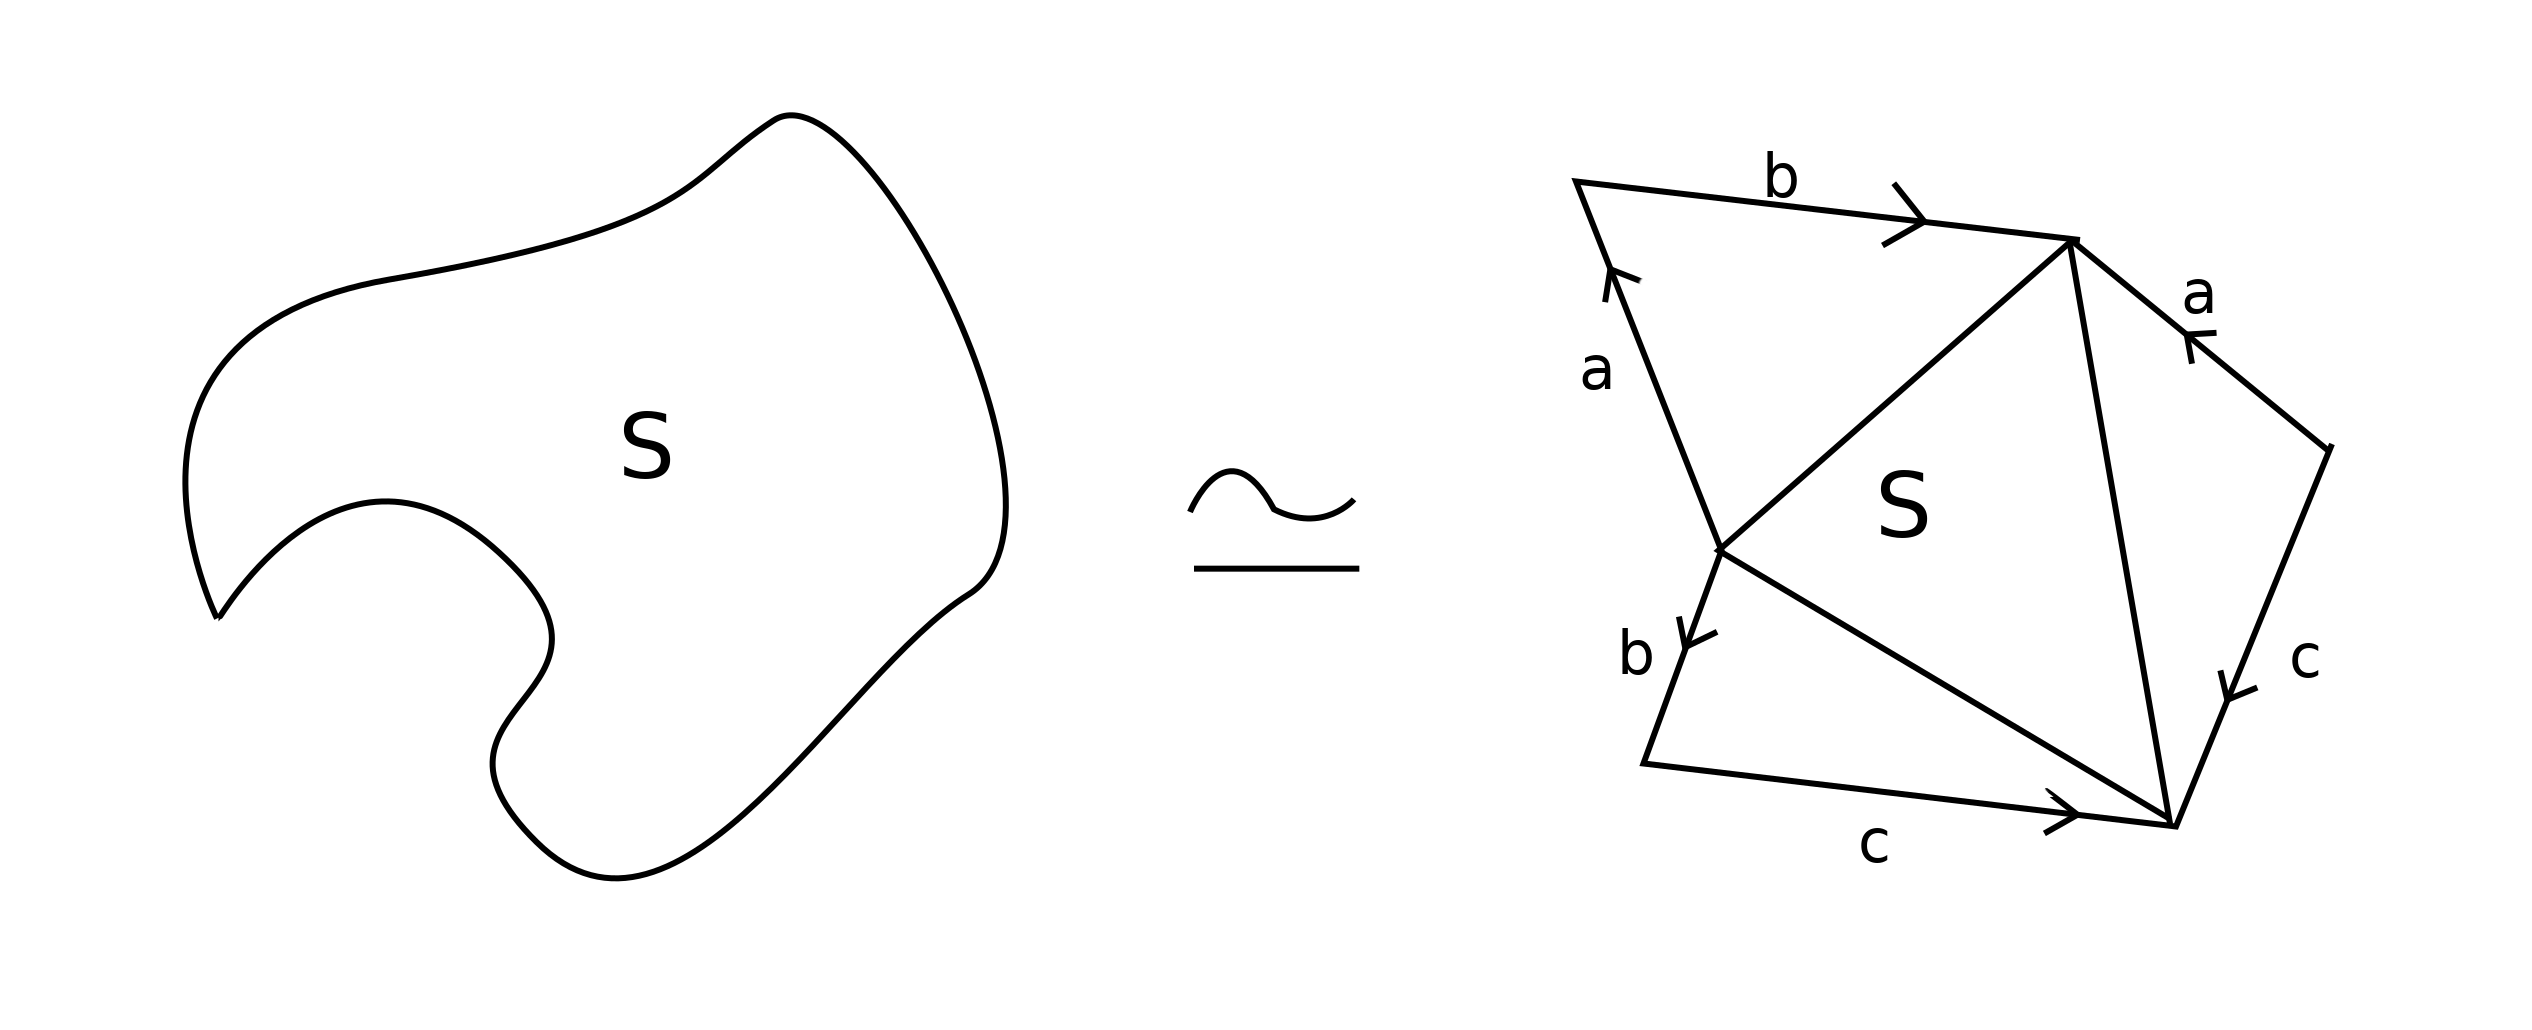
\includegraphics[width=2.3in,height=1.3in]{imagenes/paso1.png} 
\end{center}
\end{figure}
\end{block}

 
\end{frame}


% Diapo 8

\begin{frame}
\frametitle{Idea de la demostración}
\begin{block}{Paso 2}
Se realizan cortes e identificaciones para obtener un nuevo polígono equivalente a una esfera o a una suma conexa de $n$ toros.


\begin{figure}[htb]
\begin{center}
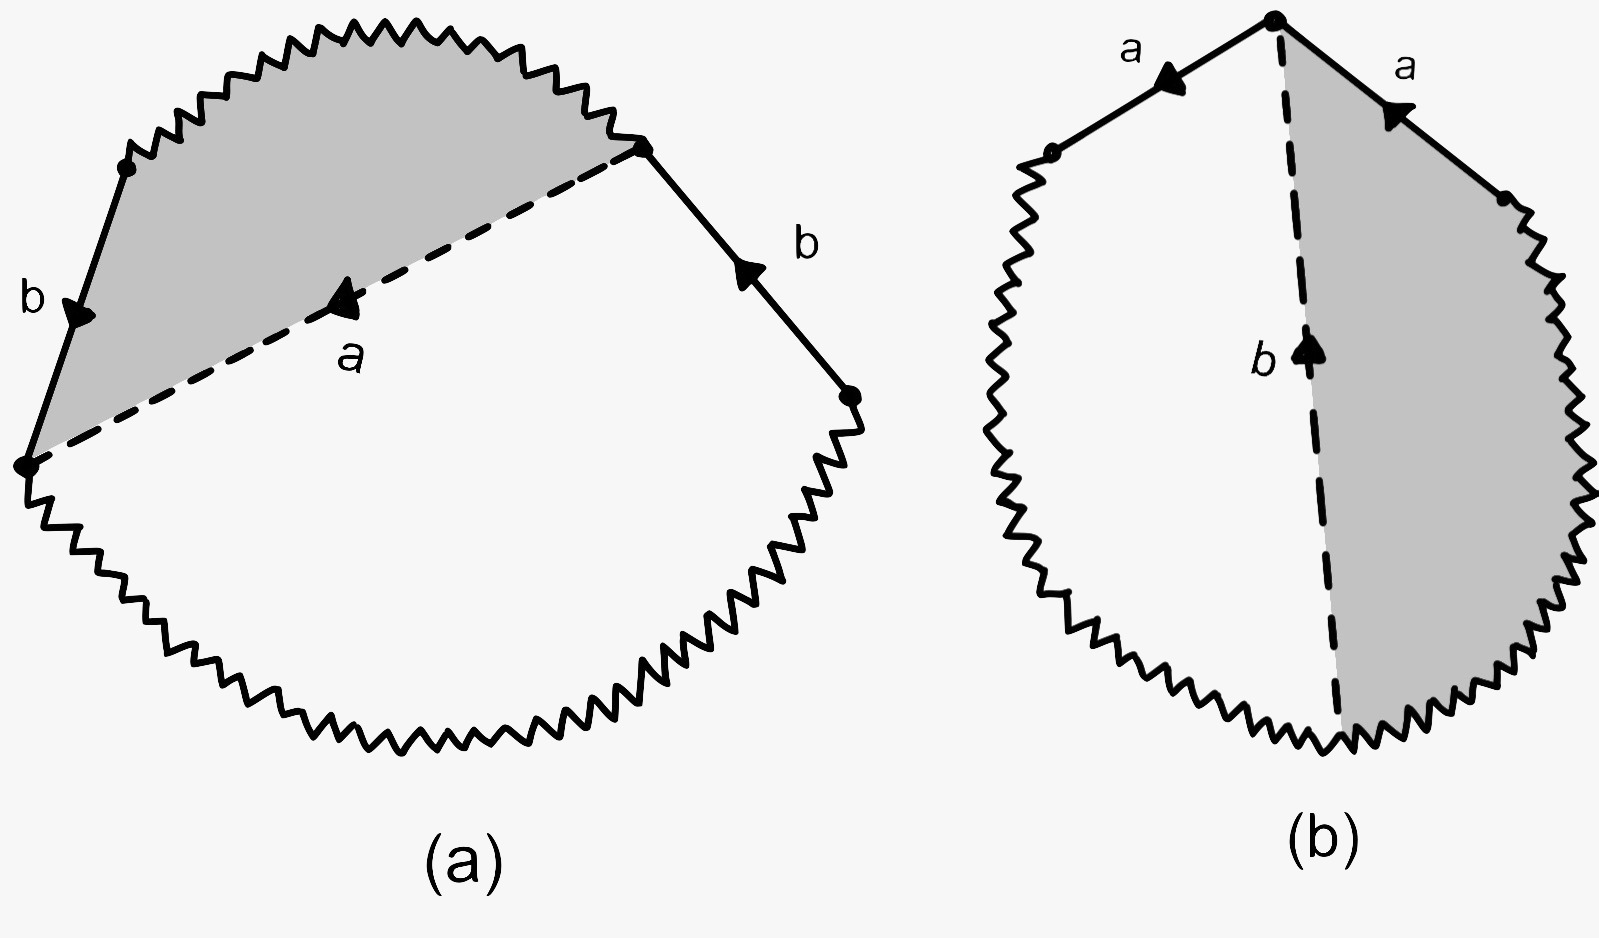
\includegraphics[width=1.5in,height=0.75in]{imagenes/paso4.jpeg} 
\end{center}
\end{figure}

\end{block}
 
\end{frame}


% Diapo 9
\begin{frame}
\frametitle{Género}
\begin{block}{Género}
Número de toros al que una superficie es homeomorfo.
\end{block}
\begin{figure}[htb]
\begin{center}
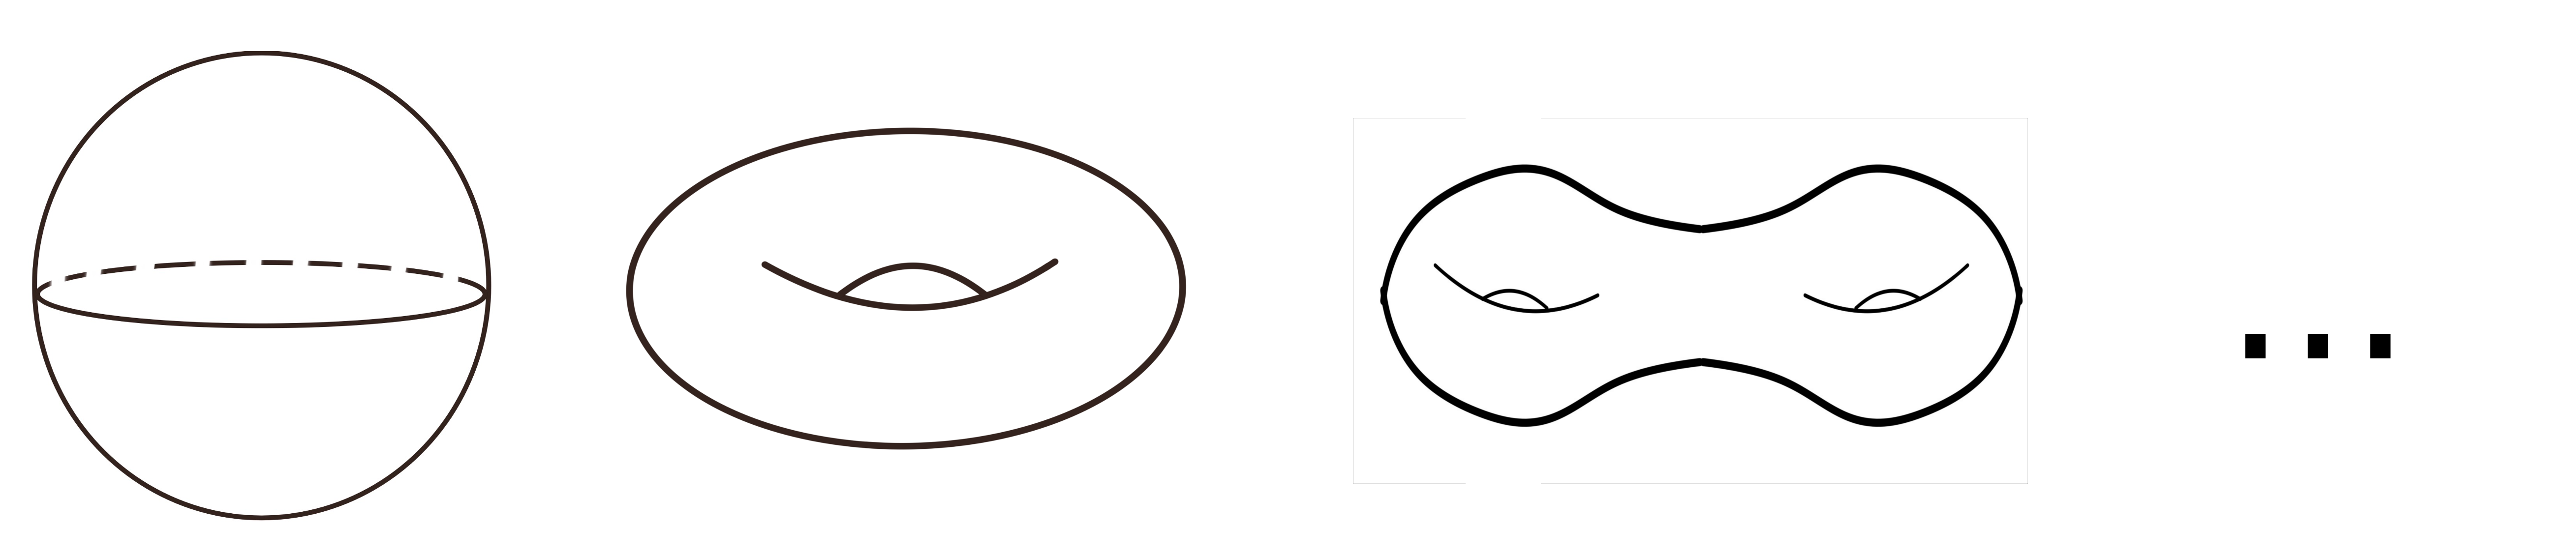
\includegraphics[width=4in,height=0.75in]{imagenes/diapo4.png} 
\end{center}
\end{figure}

\end{frame}

% Diapo 10
\begin{frame}
\frametitle{Superficies no compactas}

Ejemplos de superficies no compactas
\begin{figure}[htb]
\begin{center}
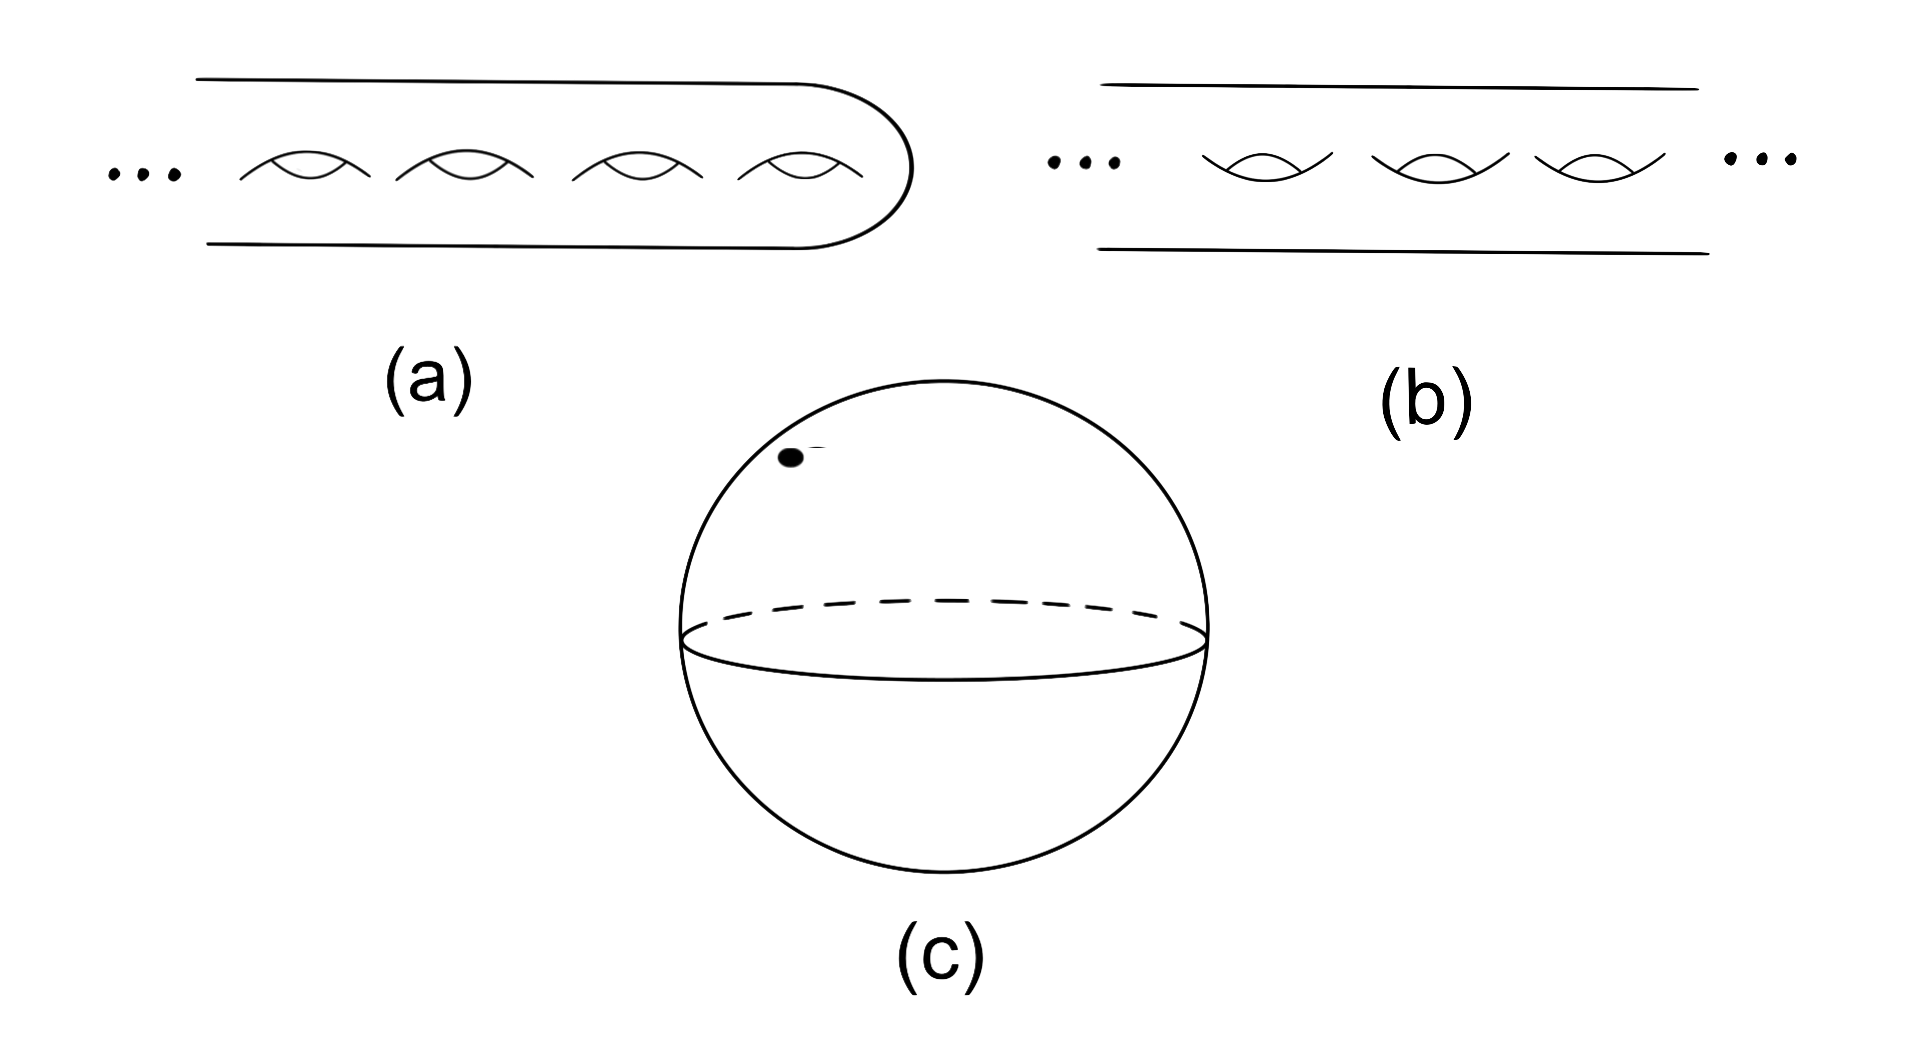
\includegraphics[width=3.3in,height=1in]{imagenes/ejemplonocompactas.png} 
\end{center}
\end{figure}


\end{frame}

% Diapo 11
\begin{frame}
\frametitle{Borde ideal}
\begin{block}
{Extremo}
Subconjuntos $P_1 \supset P_2 \supset ...$ que cumplen:
\begin{itemize}
\item Conexos, no acotados y de frontera compacta
\item $\forall A\subset S$ compacto, $\exists n$ con $P_n \cap A = \emptyset$.
\end{itemize}

\begin{figure}[htb]
\begin{center}
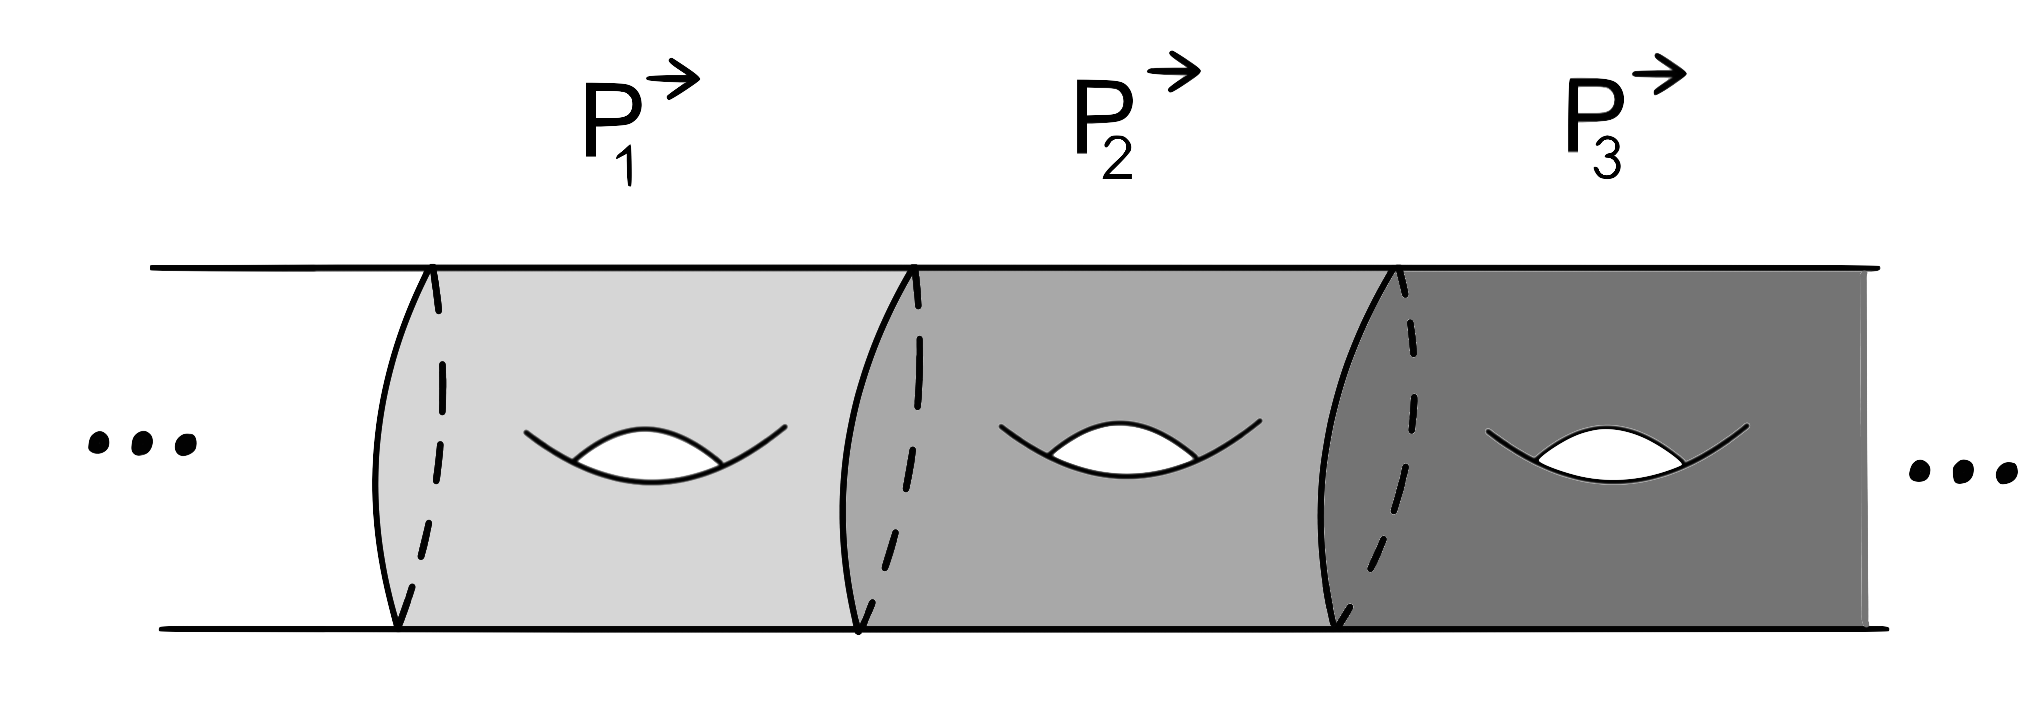
\includegraphics[width=2in,height=0.7in]{imagenes/final.png} 
\end{center}
\end{figure}
\end{block}


\begin{block}{Borde ideal}
$B(S)$ es el conjunto de extremos salvo equivalencia.
\end{block}
\end{frame}


% Diapo 12
\begin{frame}
\frametitle{Borde ideal}
\begin{block}
{Topología de B(S)}
Para $U \subset S$ no acotado de frontera compacta, definimos $U^*$ como el conjunto de extremos contenidos en $U$. 
\begin{figure}[htb]
\begin{center}
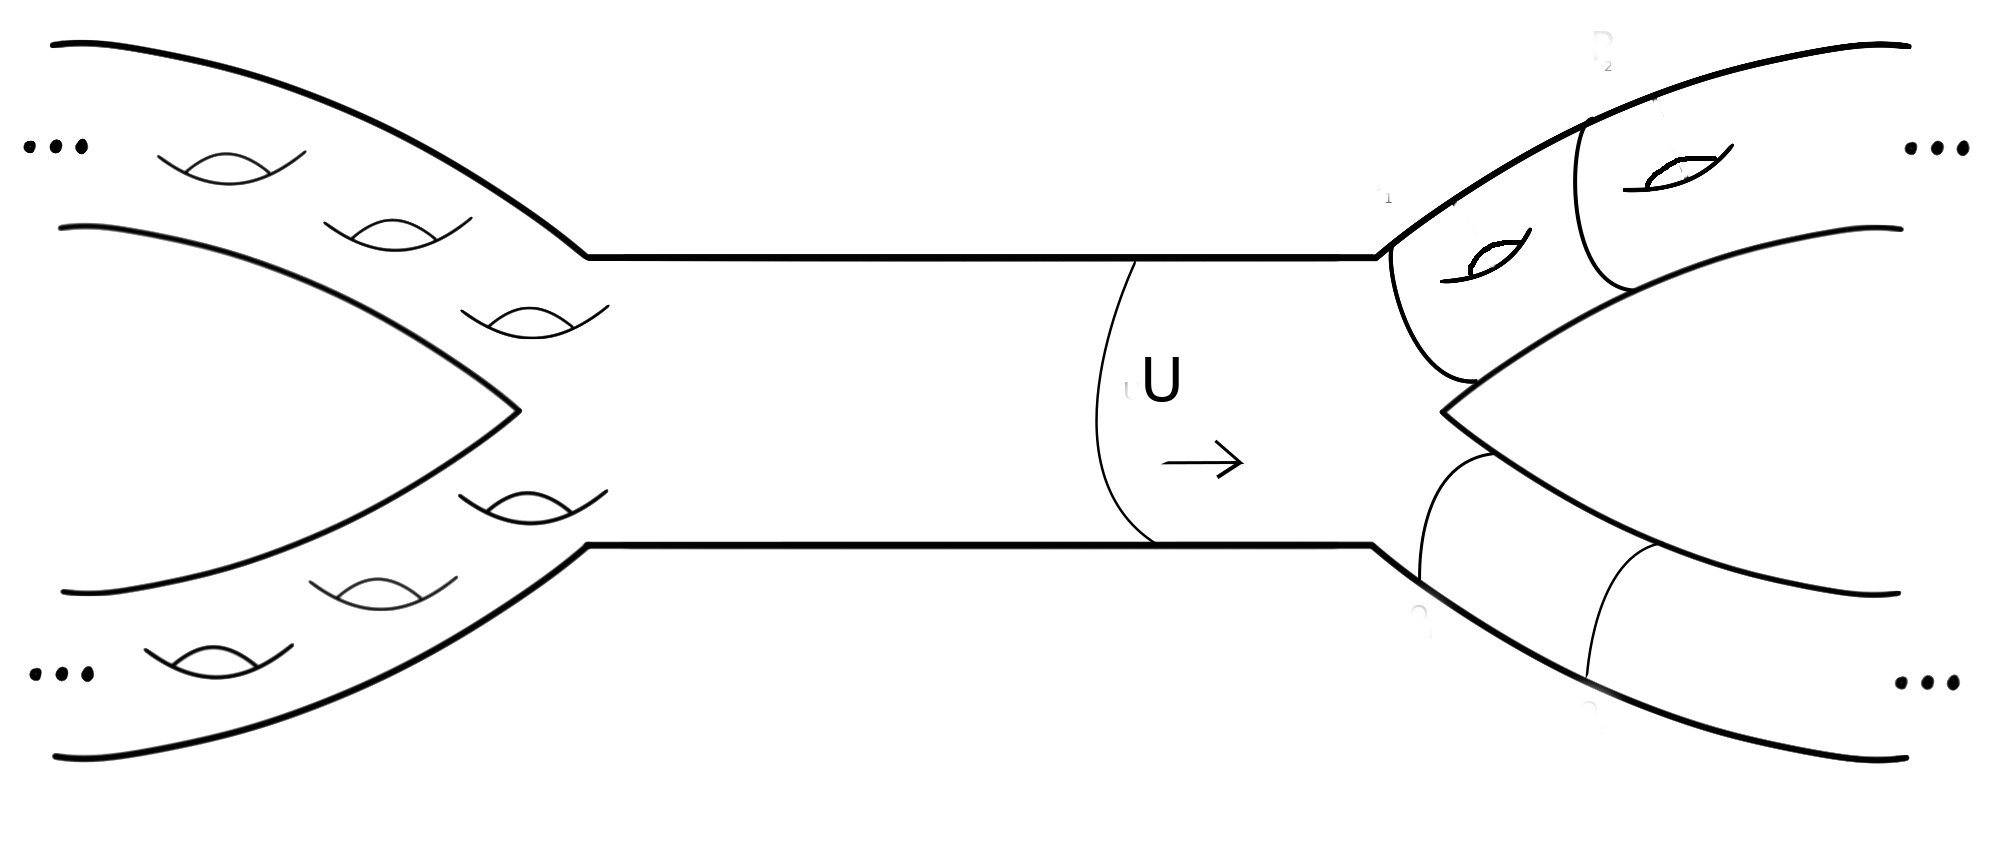
\includegraphics[width=2.5in,height=0.75in]{imagenes/diapoX.png} 
\end{center}
\end{figure}

Los $U^*$ forman una base.
\end{block}

\end{frame}

% Diapo 13
\begin{frame}
\frametitle{Tipos de extremo}

Los extremos pueden ser de género infinito o planos.
\begin{figure}[htb]
\begin{center}
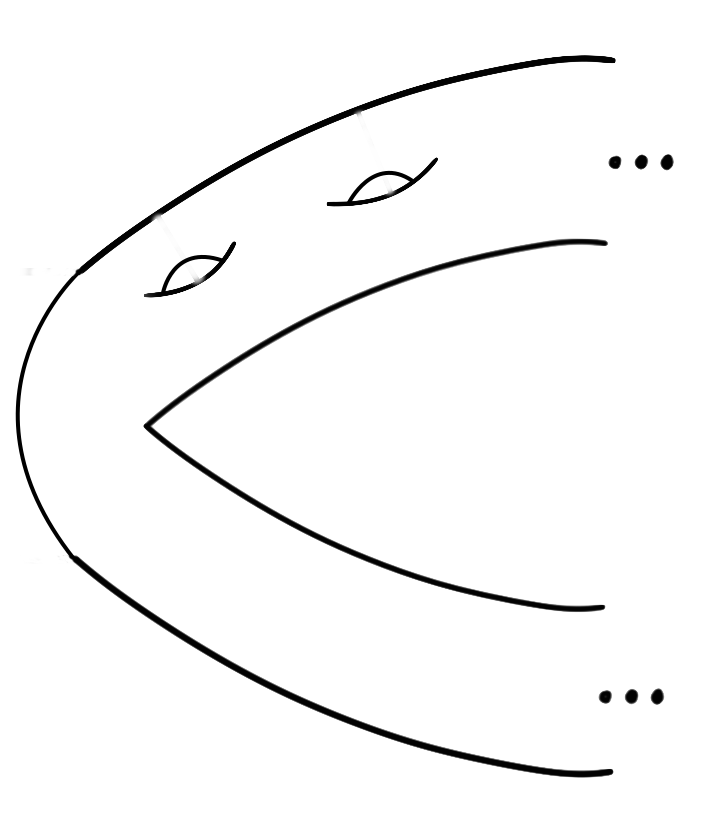
\includegraphics[width=1.2in,height=0.75in]{imagenes/dosfinales.png} 
\end{center}
\end{figure}

El conjunto $B'(S)$  de extremos de género infinito es un cerrado. Llamamos borde ideal a la tupla $(B(S), B'(S))$.
\end{frame}
 

% Diapo 14
\begin{frame}
\frametitle{Clasificación de superficies no compactas}

\begin{block}{Teorema (Kerékjártó 1923)}
El tipo topológico de una superficie orientable está determinado por su género y borde ideal.
\end{block}
\end{frame}

% Diapo 15
\begin{frame}

\frametitle{Idea de la demostración}
Se construyen inductivamente las tuplas $(A_i, A'_i, f_i)$ con:
\begin{itemize}
\item $A_i$ y $A'_i$  subsuperficies compactas.
\item $S = \bigcup_{i=0}^{\infty}A_i$  (igual con $S'$).
\item $f_i: A_i \longrightarrow A'_i$ homeomorfismo.
\end{itemize}

\end{frame}

% Diapo 16
\begin{frame}
\frametitle{Representantes de superficies no compactas}
\begin{prop}
El borde ideal de toda superficie es homeomorfo a un par (X,Y):
\begin{itemize}
\item X subconjunto cerrado del conjunto de Cantor.
\item Y cerrado de X.
\end{itemize} 
\end{prop}


\end{frame}

% Diapo 17
\begin{frame}
\frametitle{Representantes de superficies no compactas}

\begin{block}
{Teorema (Richards 1963)}
Para todo par $(X,Y)$ anterior, podemos construir una superficie con ese borde ideal.
\end{block}
\begin{block}
{Idea de la demostración}
\begin{figure}[htb]
\begin{center}
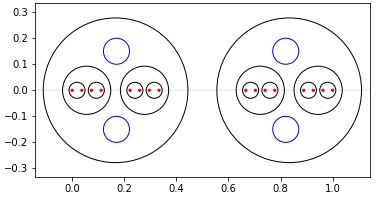
\includegraphics[width=2.5in,height=1.5in]{imagenes/eleccionCK.png} 
\end{center}
\end{figure}


\end{block}
\end{frame}



%Diapo 18
\begin{frame}
\frametitle{Cardinalidad}
Cardinalidad de superficies salvo homeomorfismo:
\begin{itemize}
\item Hay $\aleph_0$ superficies compactas.
\item Hay $2^{\aleph_0}$ superficies no compactas.
\item  Hay $2^{2^{\aleph_0}}$ superficies \textbf{no} segundo numerables.
\end{itemize}



\end{frame}

 

 
 
 
 
\end{document}




